\section{Results and discussion}\label{results}
This section presents the results of the Austrian case study. \added{Particularly, the mix of heat sources/generation technologies and related district heating networks in the four different scenarios (section \ref{res:1}) are presented.} \deleted{Four different storylines are investigated, covering a wide range of possible future developments of the Austrian energy system in the context of European deep decarbonization.} \deleted{Section \ref{res:1} shows the heat generation mix supplying the heat demand (residential and commercial) at the country level.} Section \ref{res:2} \replaced{presents the heat generation mix on the country, sub-regional and community levels.}{the heat generation mix obtained on a more granular geographical scale, at sub-regional and community levels.} Potentials of \replaced{district heating networks}{a centralized heat network´} are presented further in section \ref{res:3}. Section \ref{res:4} shows \replaced{district heating networks}{the centralized heat networks} at the community level. \replaced{Furthermore}{Finally}, section \ref{res:5} compares the projected \replaced{district heating}{centralized heat} networks in 2050 with today's networks, based on heat density. \added{Finally, section \ref{sens:hp} presents a sensitvity analysis of the allocation of heat pump (air) generation into district heating networks and its impact on the related heat densities.}

\newcolumntype{R}[2]{%
	>{\adjustbox{angle=#1,lap=\width-(#2)}\bgroup}%
	l%
	<{\egroup}%
}
\newcommand*\rot{\multicolumn{1}{R{90}{-0.5em}}}
\newcommand*\rots{\multicolumn{1}{R{90}{1em}}}
\definecolor{Gray}{gray}{0.85}

\subsection{Heat technology generation in 2050 on different spatial granularities}\label{res:2}
Figure \ref{fig:res1} shows the heat generation per technology/source on different spatial granularities: the country (NUTS0), sub-region (NUTS3), and community (LAU) levels (from left to right). The level of spatial details increases from the left to the right. In the middle, the residential and commercial heat supply in representative rural and urban sub-regions, respectively, is presented. The rural sub-region Mostviertel-Eisenwurzen (NUTS3 code AT121) shows high shares of heat pump (air \added{ and }sourced) \added{generation}\deleted{ and small-scale heat storage systems}. In addition, \replaced{biomass and direct electric}{synthetic gas and direct electric} heating systems supply the heat demand. The urban sub-region \replaced{Rheintal-Bodenseegebiet (AT342)}{\textit{South Viennese environs} (AT127)} is mainly supplied by \replaced{the same heat sources as before. Additionally, synthetic gas and waste cover heat demands. Throughout the pie charts within the figure, shares of heat generation using district heating are indicated using blue edges. On the extreme right, an example of the resulting district heating at the community level (Rheintal-Bodenseegebiet (AT342)) for the four different scenarios is presented by highlighting the supply areas. The largest supply areas of district heating are in the \textit{Gradual Development} and \textit{Techno-Friendly} scenarios. Note that the obtained district heating supply areas not necessarily are interconnected. Exemplarily, two separated communities are supplied by district heating in the \textit{Directed Transition} scenario.}{ground-sourced heat pumps, biomass, and hydrogen. Air-sourced heat pumps and, again, heat storage cover the remaining demand. Throughout the pie charts within the figure, shares of heat generation using centralized heat networks are indicated using blue edges. On the extreme right, an example of the resulting centralized heat network at the community level for the four different scenarios is presented. Within the four subfigures presenting centralized heat networks (each for one storyline), the size of the points represents the amount of heat demand using centralized supply in a community. The comparably high heat demand in the \textit{Gradual Development} scenario results in an extensive centralized heat network infrastructure (see lower right subfigure in Figure \ref{fig:res1}). The other three centralized heat networks are characterized by fewer (less supplied small sub-regions) and smaller points (less supplied heat demand by the centralized heat network). Figure \ref{fig:res-comp} compares the heat generation by source between 2020 (today) and 2050 for the four different scenarios. The height of the bars shows the absolute differences by source between both years, whereby a negative difference indicates less heat generation by this source in 2050 for the \textit{Societal Commitment} scenario. This scenario is more prominently presented as this scenario has the lowest total heat demand (-18.15TWh). In addition, the scenarios with the lowest and highest differences, respectively, are marked for each heat source and the total demand. For instance, the highest decrease is seen in natural gas in the \textit{Directed Transition} scenario (-53.76TWh).}

\begin{sidewaysfigure}
	\centering
	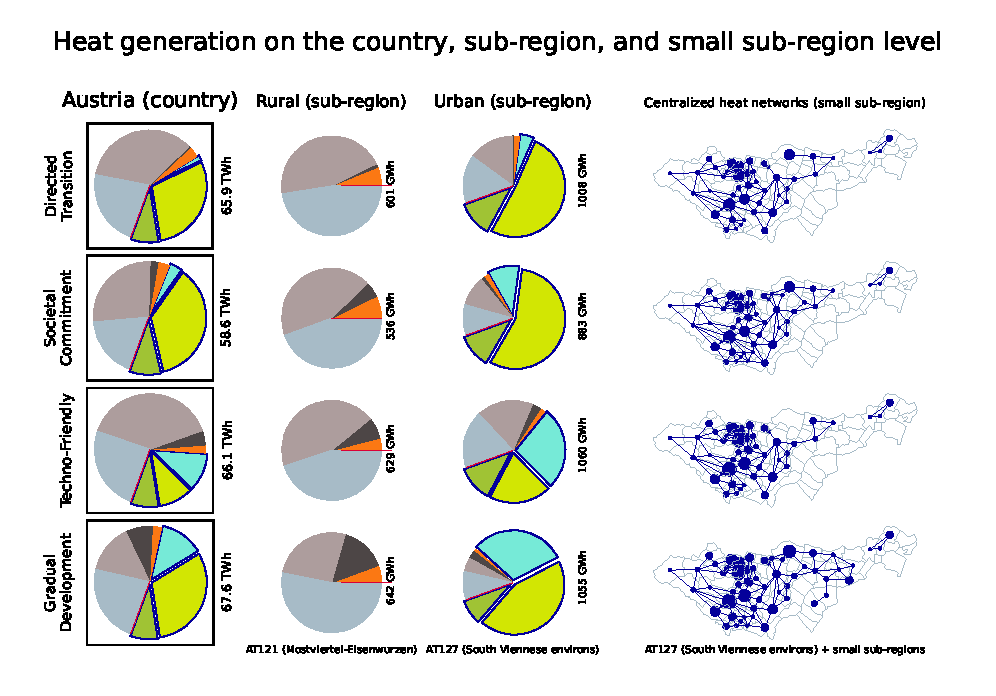
\includegraphics[width=1\linewidth]{figures/4_Results/Fig_Matrix-plot/Spatial_results.eps}
	\caption{Heat technology generation on different spatial granularity levels in the different scenarios supplying the residential and commercial heat demand. left: on the country level. middle: comparison of a rural and urban sub-region. right: \replaced{district}{centralized} heat\added{ing} \deleted{network}\replaced{supply areas}{topology (size of the points represent the amount of heat demand supplied by the network)}}
	\label{fig:res1}
\end{sidewaysfigure}

\subsection{Sub-regions in Austria 2050 with high potentials for centralized heat supply}\label{res:3}
\added{Figure \ref{fig:res2} presents heat demand supplied by district heating in Austria in 2050 on the NUTS3 level. There are four different sub-regions (AT130 Vienna, AT221 Graz, AT312 Linz-Wels and AT342 Rheintal-Bodenseegebiet) with district heating in the four scenarios. Although the four different sub-regions are the same in the four scenarios, the heat demand supplied by district heating varies significantly (see also the column district heating in Table \ref{tab:comparison}). The highest amount of district heating is in the \textit{Gradual Development} scenario. The exact numbers of district heating and on-site heat supply for the four different sub-regions and scenarios are presented in Table \ref{tab:3}. For each sub-region, the share of district heating is in the \textit{Gradual Development} the highest (between 87\% and 99\%).} \deleted{The share of district heating on the total heat supply varies among the four different scenarios. The highest shares of district heating for each sub-region are in the \textit{Gradual Development} and \textit{Techno-Friendly} scenario. The potentials for centralized heat supply in Austria in 2050 are limited to densely populated areas (urban areas). In particular, the results indicate eight different sub-regions (NUTS3 regions) that are supplied by centralized heat networks (see Figure \ref{fig:res2}). Although the exact numerical numbers differ, the eight sub-regions in each scenario are (partially) supplied by centralized heat networks. Table \ref{tab:3} shows the centralized and on-site (decentralized) heat supply in the sub-regions. Thereby, the connection rate is assessed by the share of centralized heat supply in the total heat demand. Note that the population density varies in these sub-regions between 163persons/km\textsuperscript{2} (AT211 - Klagenfurt-Villach) and 5124 persons/km\textsuperscript{2} (AT130 - Vienna).}

\begin{table} \centering
	\resizebox{0.9\textwidth}{!}{% use resizebox with textwidth
		\renewcommand{\arraystretch}{1.1}
		\begin{tabular}{cccccc}
			\toprule 
			&& \multicolumn{2}{c}{in TWh} & in \%\\\cmidrule(lr){3-4}\cmidrule(lr){5-5}
			Sub-region & Scenario&District heating (DH) & On-site & Share of DH\\\hline
			 \parbox[t]{15mm}{\multirow{4}{*}{\rotatebox[origin=c]{90}{\parbox{2cm}{\centering Vienna\\(AT130)}}}} & Directed Transition & 4.22 & 6.76 & 38\\
			 & Societal Commitment & 5.70 &  4.62 & 55\\
			 & Techno-Friendly & 10.11 &  0.58 & 95\\
			 & Gradual Development & 11.12 &  0.07 & 99\\\hline
			  \parbox[t]{15mm}{\multirow{4}{*}{\rotatebox[origin=c]{90}{\parbox{2cm}{\centering Graz\\(AT221)}}}} & Directed Transition & 0.38 & 2.17 & 15\\
			 & Societal Commitment & 0.60 &  1.80 & 25\\
			 & Techno-Friendly & 1.34 & 1.14 & 54\\
			 & Gradual Development & 2.25 & 0.35 & 87\\\hline
			 \parbox[t]{15mm}{\multirow{4}{*}{\rotatebox[origin=c]{90}{\parbox{2cm}{\centering Linz-Wels\\(AT312)}}}} & Directed Transition & 0.51 & 2.91 & 15\\
			 & Societal Commitment & 0.80 & 2.42 & 25\\
			 & Techno-Friendly & 1.80 & 1.53 & 55\\
			 & Gradual Development & 3.03 & 0.46 & 87\\\hline
			 \parbox[t]{15mm}{\multirow{4}{*}{\rotatebox[origin=c]{90}{\parbox{2cm}{\centering Rheintal-Bodensee\\(AT342)}}}} & Directed Transition & 0.27 & 1.54 & 15\\
			 & Societal Commitment & 0.42 & 1.28 & 25\\
			 & Techno-Friendly & 0.96 & 0.81 & 54\\
			 & Gradual Development & 1.60 & 0.25 & 86\\
			\bottomrule
	\end{tabular}}
	\caption{Heat demand supplied by district heating and on-site (incl. share of district heating of total heat supply) in the four Austrian sub-regions in 2050.}
	\label{tab:3}
\end{table}

\begin{sidewaysfigure}
	\centering
	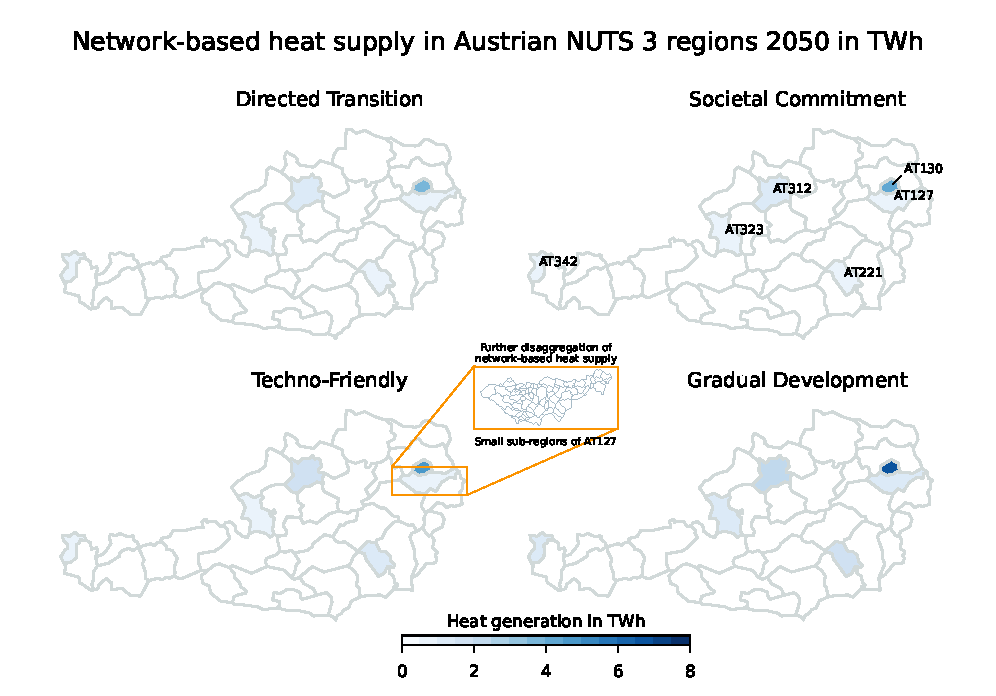
\includegraphics[width=1\linewidth]{figures/4_Results/Fig-Heatmap/Heatmap.eps}
	\caption{Heat demand supplied by centralized heat networks in Austria 2050. The white areas are supplied by on-site (decentralized) sustainable heat generation technologies/sources.}
	\label{fig:res2}
\end{sidewaysfigure}

\subsection{\replaced{District}{Centralized} heat\added{ing} network topology at the community level}\label{res:4}
This section presents the \replaced{district}{centralized} heat\added{ing} network topology of the sub-region \replaced{\textit{Linz-Wels} (AT312)}{\textit{South Viennese environs} (AT127)} and all included communities \added{in the \textit{Directed Transition} scenario}. \deleted{In Figure \ref{fig:res2}, this particular sub-region is marked by the orange box.} Figure \ref{fig:res3} shows the projected \replaced{district heating supply area}{centralized heat network topology}. In particular, the network topology is presented for the initial condition (as a result of the sequential downscaling, $i=1$) and the final condition of the network \added{(as a result of the iterative downscaling}, $i=65$). The distribution of the benchmark indicator values of the \replaced{district}{centralized} heat\added{ing} network depending on the number of iterations is presented in the middle. The \replaced{median}{mean value} is marked in orange. The supply area decreases with an increasing number of iterations. In the community analysed here, the termination criterion of the algorithm is reached when \replaced{10}{25} communities are connected (starting from \replaced{74}{75} in the initial condition). The number of connected population decreases by \SI{40}{\%}, starting from a population of \SI{663,000}{} being connected \added{(or rather having access since the in general the connection rate to district heating is not equal to one in the initial condition)} to the \replaced{district}{centralized} heating network in the initial condition. After the final iteration ($i=65$), the termination criterion is reached. \deleted{Note that the iterative reduction of small sub-regions supplied does not necessarily result in one contiguous network.}

\begin{sidewaysfigure}
	\centering
	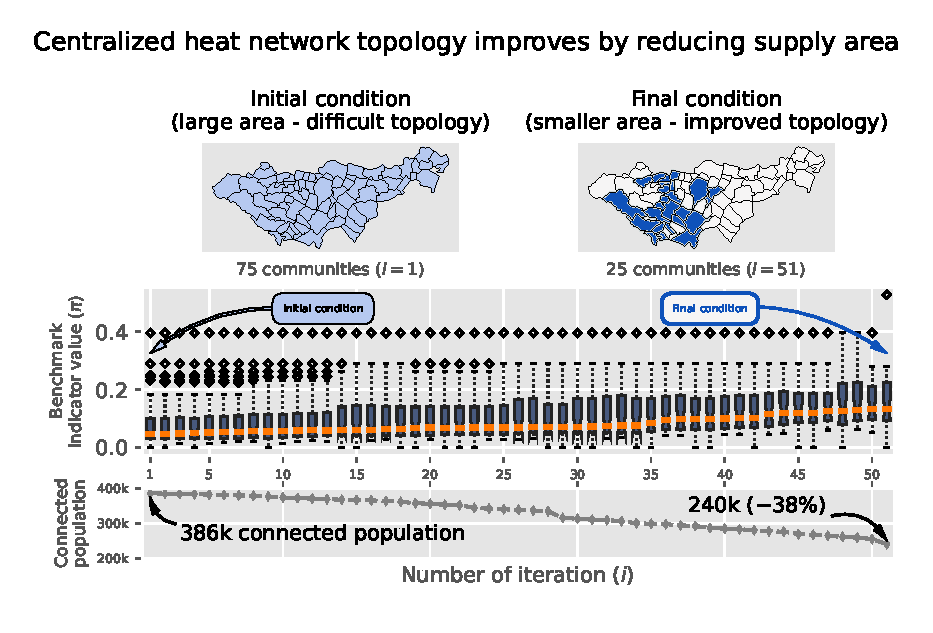
\includegraphics[width=1\linewidth]{figures/4_Results/Fig_Boxplot/ext_boxplot.eps}
	\caption{\replaced{District}{Centralized} heat\added{ing} network topology \replaced{in Linz-Wels (AT312) in the \textit{Directed Transition} scenario}{in the initial and final condition}. The boxplot (middle) indicates the improved network topology by \deleted{an} increasing benchmark indicator \replaced{values}{mean value (orange line)}. In the final condition \added{10 communities; i=65}, the \replaced{population of connected communities}{connected population} declines by \SI{-40}{\%} compared to the initial condition (74 communities; i=1).}
	\label{fig:res3}
\end{sidewaysfigure}

\subsection{Comparison of 2050's and today's \replaced{district}{centralized} heat\added{ing} networks using heat density as a criteria}\label{res:5}
In the following, the \replaced{district}{centralized} heat\added{ing} network in \replaced{Linz-Wels (AT312)}{\textit{Graz} (AT221)} is shown in detail. This area is selected for illustrative purpose, because it provides representative results in terms of both the applied downscaling and achievable heat density benchmarks of centralized heat networks. Figure \ref{fig:res5} shows the heat density of \replaced{district heating}{the centralized heat network} in the \textit{Techno-Friendly} scenario.

\begin{figure}[h]
	\centering
	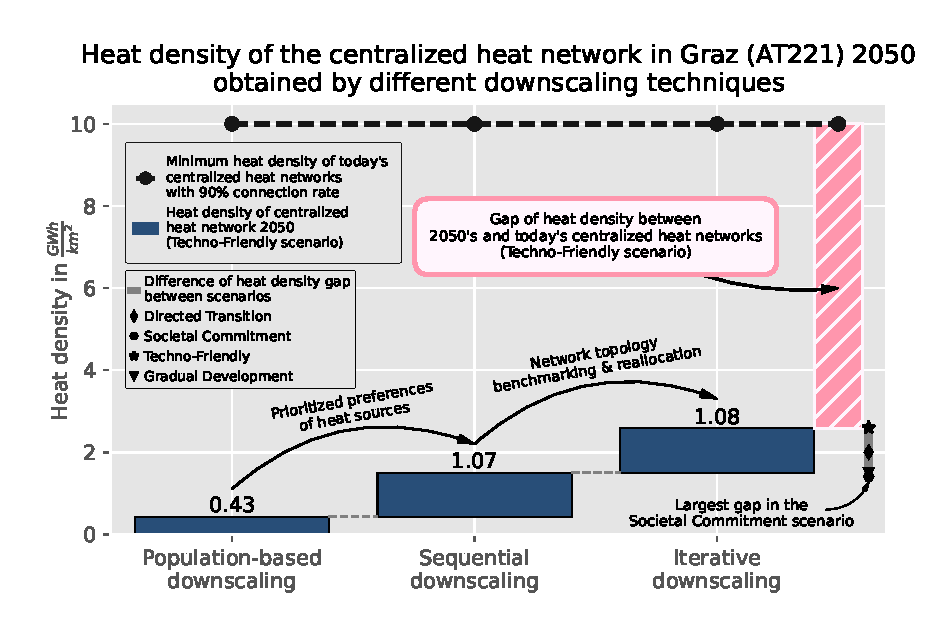
\includegraphics[width=0.9\linewidth]{figures/4_Results/Fig_Heat-density/HD_cleaned1.eps}
	\caption{Heat density of the \replaced{district}{centralized} heat\added{ing} \deleted{network} in \replaced{Linz-Wels (AT312)}{\textit{Graz} (AT221)} 2050 in the \textit{Techno-Friendly} scenario. The gap of heat density between 2050s and today (black dashed line) is marked by the pink bar.}
	\label{fig:res5}
\end{figure}

The x-axis shows the three different downscaling techniques. The numerical numbers indicate a significant increase of the heat density by the sequential (+\SI{0.49}{GWh \per km^2}) and, in particular, the iterative downscaling (+\SI{3.21}{GWh \per km^2}). However, comparing the heat density value obtained with the heat density values of today's centralized heat networks reveals a significant gap (see the hatched pink bar). Here, in the \textit{Techno-Friendly} scenario, it is \SI{5.75}{GWh \per km^2}. According to references from the practice (\deleted{see, e.g., in}\url{http://www.austrian-heatmap.gv.at/ergebnisse/}), the \added{threshold} heat density of today's networks is assumed to be \SI{10}{\frac{GWh}{km^2}} with a connection rate of \SI{90}{\%}. The gap of heat density varies between the different scenarios. \added{This is shown in detail below.}
%\deleted{Figure \ref{fig:res4} shows the heat densities in the sub-regions and compares the results in the different scenarios. It shows the scenarios with the lowest and highest heat densities. The bottom bar shows the value and scenario with the lowest heat density among the four different scenarios for each sub-region. The hatched bar indicates the increase of heat density and the corresponding scenario compared to the lowest value.}\replaced{In Vienna (AT130), the heat density is in each scenario higher than}{In five sub-regions, the \textit{Techno-Friendly} scenario is the scenario with the lowest heat density. The \textit{Directed Transition} scenario is the scenario with the highest heat density in four sub-regions. Note that Vienna (AT130) is not shown for the sake of clarity. The heat density there varies between 15.1 GWh/km\textsuperscript{2} in the \textit{Techno-Friendly} and 30.3 GWh/km\textsuperscript{2} in the \textit{Gradual Development} scenario.} \SI{10}{GWh \per km^2} \added{and is maximal} \SI{27}{GWh \per km^2} \added{in the \textit{Gradual Development} scenario. In Linz-Wels (AT312), the maximal heat density is} \SI{7.7}{GWh \per km^2} \added{in the \textit{Societal Commitment} scenario. The two sub-regions Graz (AT221) and Rheintal-Bodensee (AT342) reach their maximum heat densities in the \textit{Techno-Friendly} scenario with} \SI{6.1}{GWh \per km^2} \added{and} \SI{3.8}{GWh \per km^2} \added{respectively. Three sub-regions (Vienna (AT130), Graz (AT221) and Rheintal-Bodensee (AT342)) have their lowest heat density in the \textit{Directed Transition} scenario which has the lowest amount of district heating compared to the others (compare Table \ref{tab:comparison}). At the same time, the three sub-regions have their highest heat density in the \textit{Gradual Development} and \textit{Techno-Friendly} scenario which both have the highest amount of district heating. The sub-region Linz-Wels (AT312) has its minimum heat densitiy in the \textit{Gradual Development} and its maximum in the \textit{Societal Commitment} scenario. The latter scenario is characterized by a comarable low amount of district heating (Table \ref{tab:comparison}).}
 
%\begin{figure}[h]
%	\centering
%	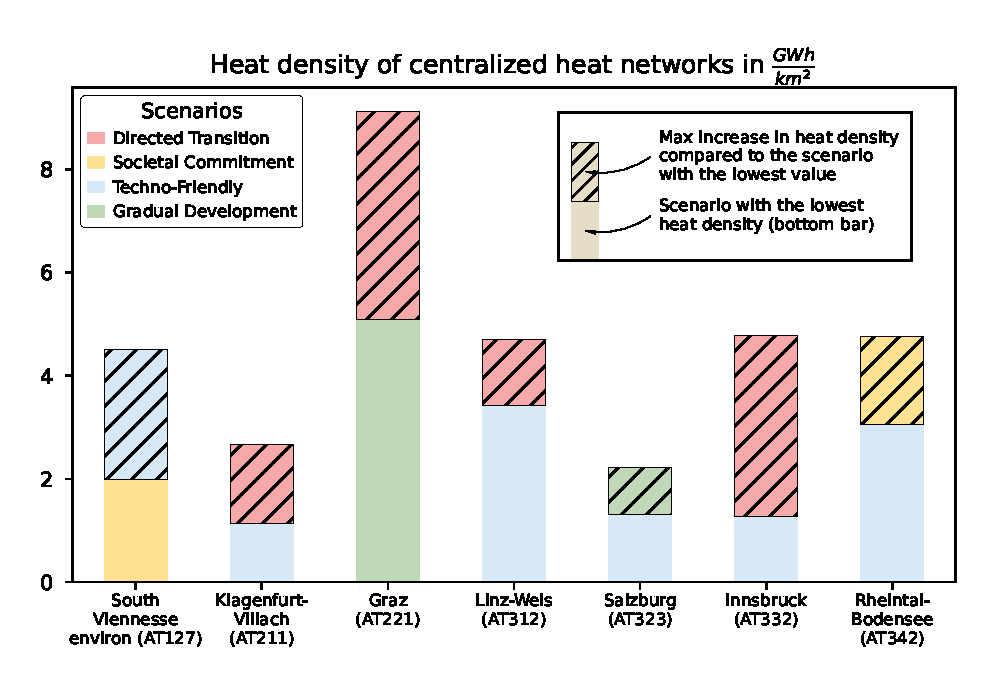
\includegraphics[width=1\linewidth]{figures/4_Results/Fig_benchmark/benchmark.eps}
%	\caption{Comparison of the heat density per sub-region in the four different scenarios. The bottom bar shows the scenario with the lowest heat density. The hatched bar indicates the increase of heat density and the corresponding scenario compared to the lowest value.}
%	\label{fig:res4}
%\end{figure}

\subsection{Allocation of heat pump (air) heat generation to district heating}\label{sens:hp}
\added{Building upon Figure \ref{fig:res5}, it is evident that the heat density of district heating varies significantly among the different scenarios. Moreover, the district heating networks of some sub-regions reach their highest values in scenarios with low (e.g., Linz-Wels (AT312)) and some in scenarios with high district heating shares (e.g., Graz (AT221)) on total heat supply. Accordingly, this section examines the impact of increasing shares of heat pump (air) heat generation feeding into district heating on the heat densitiy of district heating networks. Hence, a sensitivity analysis is carried out varying the proportion of large-scale (i.e. feeding into district heating) and small-scale (i.e. on-site heat generation) heat pump (air) generation on the downscaled values}\footnote{\added{See Figure \ref{fig:sens}} in \ref{Appendix:D}.}. \added{Figure \ref{fig:max_heat_densities} shows the heat density of district heating networks in the four different sub-regions and scenarios. Therein, the range of heat density resulting from different shares of large-scale and small-scale heat pump (air) generation is presented. The two extreme points namely that only small-scale or large-scale heat pump (air) units are used in the sub-regions are marked by the black circle (i.e. heat pump (air) on-site) and diamond (i.e. heat pump (air) in district heating). Particularly, the heat density in the \textit{Directed Transition} and \textit{Societal Commitment} scenario increase significantly compared with on-site heat pump (air) generation only (e.g. in Graz (AT221) and Linz-Wels (AT312)). In Linz-Wels, for example, this maximum is reached by two thirds large-scale heat pump (air) generation feeding into district heating}\footnote{\added{See again Figure \ref{fig:sens} (bottom) where the orange bar indicates the share of large-scale heat pump (air) generation at which the heat density is reaching its maximum.}}. \added{In Vienna (AT130), the heat density remains almost the same in the \textit{Techno-Friendly} and \textit{Gradual Development} scenario. At the same time, the heat density there increases and reaches} \SI{18}{GWh \per km^2} \added{in the \textit{Directed Transition} and \textit{Societal Commitment} scenario. In Rheintal-Bodensee (AT342), the heat densities are relatively low compared to the others independently of the allocation of heat pump (air) generation to district heating.}

\begin{figure}[h]
	\centering
	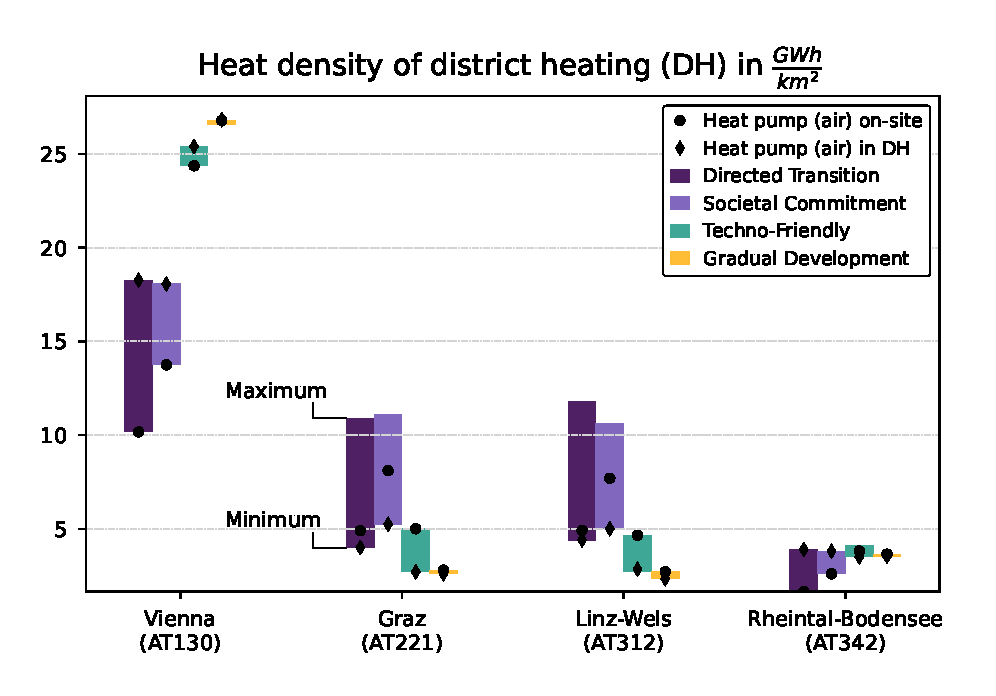
\includegraphics[width=1\linewidth]{figures/4_Results/Max_Heatdensity/4x4.eps}
	\caption{\added{Heat density of district heating in the four different sub-regions and scenarios in 2050 for varying shares of heat pump (air) generation in district heating.}}
	\label{fig:max_heat_densities}
\end{figure}